\documentclass[a4paper,oneside,12pt]{article}

\usepackage[slovene]{babel}    % slovenian language and hyphenation
\usepackage[utf8]{inputenc}    % make čšž work on input
\usepackage[T1]{fontenc}       % make čšž work on output
\usepackage[reqno]{amsmath}    % basic ams math environments and symbols
\usepackage{amssymb,amsthm}    % ams symbols and theorems
\usepackage{url}               % \url and \href for links
\usepackage{icomma}            % make comma a thousands separator with correct spacing
\usepackage{graphicx}          % slike
\usepackage{enumitem}          % seznami
\usepackage[bookmarks, colorlinks=true, linkcolor=black, anchorcolor=black,
  citecolor=black, filecolor=black, menucolor=black, runcolor=black,
  urlcolor=black, pdfencoding=unicode]{hyperref}  % clickable references, pdf toc
\usepackage[
  paper=a4paper,
  top=2.5cm,
  bottom=2.5cm,
  left=2.5cm,
  right=2.5cm
% textheight=24cm,
% textwidtht=16cm,
]{geometry}  % page geomerty

\pagestyle{empty}              % vse strani prazne
\setlength{\parindent}{0pt}    % zamik vsakega odstavka
\setlength{\parskip}{10pt}     % prazen prostor po odstavku
\setlength{\overfullrule}{30pt}  % oznaci predlogo vrstico z veliko črnine

\newenvironment{enumerate*}{\vspace{-1\parskip}\begin{enumerate}\setlength{\itemsep}{0pt}\setlength{\parskip}{2pt}}{\end{enumerate}\vspace{-1\parskip}}
\newenvironment{itemize*}{\vspace{-1\parskip}\begin{itemize}\setlength{\itemsep}{0pt}\setlength{\parskip}{2pt}}{\end{itemize}\vspace{-2.3\parskip}}

\begin{document}

\begin{minipage}[t]{0.7\linewidth}
Študentski svet Fakultete za matematiko in fiziko \\
Jadranska 19 \\
1000 Ljubljana \\

Ljubljana, \today\\
\end{minipage}%
\begin{minipage}[t]{0.3\linewidth}
  \mbox{} \\[-15pt]
  \hspace*{\fill} 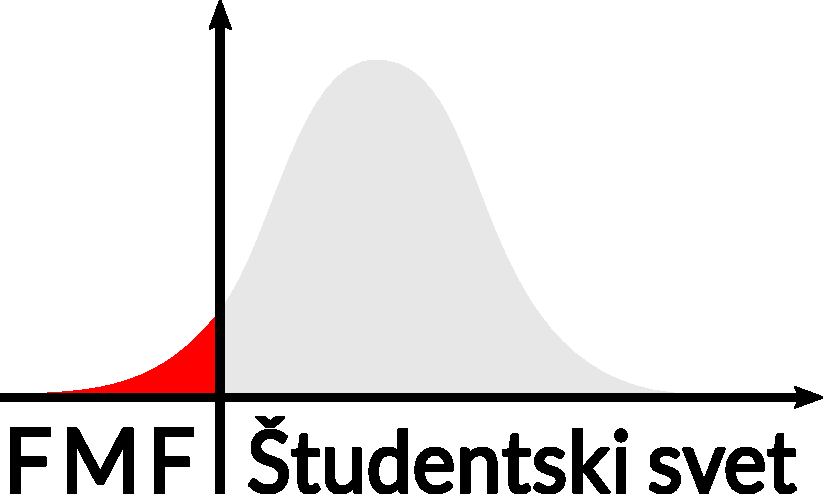
\includegraphics[width=0.9\linewidth]{ssfmf_logo_col.pdf}
\end{minipage}

Fakulteta za matematiko in fiziko \\
Jadranska 19 \\
1000 Ljubljana \\

\textbf{ZADEVA: Pridobitev certifikata LGBT prijazno}

Med študenti se je pojavila ideja, da bi FMF zaprosil za certifikat LGBT prijazno\footnote{http://www.ljubljana.si/si/zivljenje-v-ljubljani/lgbt/}.
V študentskem svetu se strinjamo s to pobudo, saj se nam zdi pomembno, da se znotraj
fakultete in tudi navzven ustvari klima, ki je pozitivna in vključujoča za vse. S tem
certifikatom bi tako pripomogli k boljšemu vzdušju na
fakulteti in skrbeli, da se ohranja in širi ideja o enakem pristopu do vseh ljudi ter
zagotavljali upoštevanje temeljnih človekovih pravic med zaposlenimi in študenti.
Študentski svet tako predlaga vodstvu fakultete, da FMF pridobi certifikat
LGBT prijazno in s tem pripomore k še boljšemu študijskemu okolju.

Lep pozdrav, \\
\hspace*{\fill} Jure Slak  \\
\hspace*{\fill} Predsednik ŠS FMF

\end{document}
